\chapter{Results}

\section{Baseline Model Performance}

The summary of the baseline comparison results in Table~\ref{tab:baseline_comparison} provides insight into the performance of each architecture family, without fusion, on the Base dataset, evaluated using the defined classification metrics.

Within the used variants of the ResNet family, ResNet-18 stood out with an overall performance, achieving an \ac{auc} of 82\% and an accuracy of 82\%. 
The findings indicate that its lightweight architecture was not only competitive but also surpassed deeper models in this specific context. In contrast, ResNet-50 and ResNet-101, despite their increased depth and capacity, did not exhibit a significant advantage; in fact, their \ac{auc}, accuracy, and precision metrics were somewhat lower.
Consequently, we establish the ResNet-18 as the baseline for subsequent fusion information studies.

The EfficientNet variants demonstrated comparable results, with \ac{auc} and accuracy values consistently ranging between 79\% and 80\%. Notably, EfficientNet-B1 achieved the highest precision among the three variants at 81\%, although its sensitivity was slightly lower at 74\% compared to B0 and B2.
The findings indicate that all three EfficientNet variants demonstrated strong and consistent performance, with only minor improvements noted when scaling up the models for this dataset. Given these minor performance differences, we opted to use the least complex model, the B0 architecture, for fusion.

The ConvNeXt (Tiny), while imposing higher computational demands, achieved an \ac{auc} of 78\% and an accuracy of 79\%. These results are marginally lower than those of the leading ResNet and EfficientNet models. Its precision was similar, but the sensitivity was notably lower, indicating that the model may be less efficient at accurately identifying positive cases in its current configuration.

\begin{table}[ht]
    \centering
    \caption{Comparison of Baseline Architectures on the Base Dataset.}
    \label{tab:baseline_comparison}
    \begin{tabular}{lcccc}
        \toprule
        \textbf{Model} & \textbf{AUC} & \textbf{Accuracy} & \textbf{Precision} & \textbf{Sensitivity} \\
        \midrule
        ResNet-18         & \textbf{0.82 ± 0.01} & \textbf{0.82 ± 0.02} & \textbf{0.82 ± 0.05} & 0.77 ± 0.04 \\
        ResNet-50         & 0.81 ± 0.02 & 0.81 ± 0.02 & 0.80 ± 0.05 & 0.78 ± 0.07 \\
        ResNet-101        & 0.79 ± 0.02 & 0.80 ± 0.02 & 0.76 ± 0.04 & \textbf{0.79 ± 0.05} \\ \hline \addlinespace
        EfficientNet-B0   & 0.80 ± 0.03 & 0.80 ± 0.03 & 0.78 ± 0.04 & 0.76 ± 0.07 \\
        EfficientNet-B1   & 0.80 ± 0.03 & 0.80 ± 0.04 & 0.81 ± 0.08 & 0.74 ± 0.05 \\
        EfficientNet-B2   & 0.79 ± 0.04 & 0.79 ± 0.04 & 0.77 ± 0.06 & 0.76 ± 0.07 \\ \hline \addlinespace
        ConvNeXt-Tiny     & 0.78 ± 0.02 & 0.79 ± 0.02 & 0.79 ± 0.03 & 0.71 ± 0.06 \\		
        \bottomrule
    \end{tabular}
\end{table}

The results indicate that lighter-weight architectures may perform competitively in lung nodule classification on the \ac{lidc-idri} dataset, achieving balanced performance across all metrics. In contrast, deeper or more complex models did not show significant improvements in performance and, in some instances, even performed worse. The inferior performance of deeper models may be explained by the relatively small size of the \ac{bb}, which may not provide sufficient spatial context for deeper architectures to leverage their increased capacity effectively. This emphasizes the need to tailor model complexity to the specific dataset and task. Since ResNet-18 yielded the best results, we used it as the foundation for our feature fusion analyses.

\FloatBarrier

\section{Impact of Individual Radiomics Feature Fusion}

Founded on the results retrieved from this phase, exposed in Table~\ref{tab:resnet_fusion_layers_grouped}, the systematic evaluation of individual radiomics feature fusion highlights several key trends. These trends relate to the utility of specific feature categories and the effects of the fusion stage within the ResNet-18 architecture.

Shape features consistently demonstrated the highest performance among all tested radiomics groups, achieving an \ac{auc} of up to 84\% and an accuracy of 84\% when integrated at the earliest stage of the ResNet architecture - after the first ResNet-18 block. This finding underscores the significance of shape-based descriptors, as they provide particularly valuable information for the classification task when incorporated early in the feature fusion pipeline.

Both \ac{fof} and \ac{lbp} also exhibited strong performance, particularly at the first and second fusion stages, after the first and second ResNet-18 blocks, achieving \ac{auc} scores of 83\%. This underscores the importance of basic intensity and texture information in fusion when fusion occurs at an earlier stage. 
On the other hand, \ac{hog}, Gabor, and Haralick features produced slightly lower, yet still robust results, with \acp{auc} in the range of 80–82\% across fusion stages. While their impact was not as pronounced as that of shape features, their integration consistently enhanced or matched baseline performance.

For most feature types, the most favorable results were observed when fusion occurred after either the first or second ResNet block.
This suggests that fusion at an early stage may promote a more effective joint representation, likely because the network can more effectively propagate and refine the complementary information provided by radiomics features through subsequent layers.
 In contrast, fusion at later stages generally yielded marginally lower metrics, potentially due to reduced opportunities for the model to integrate and utilize the auxiliary features as it approached the final decision layers.

Sensitivity values showed an upward trend when fusion was also conducted at earlier stages. Precision tended to be greatest for Shape, \ac{fof}, and \ac{lbp} features during early fusion stages, demonstrating a favorable balance between false positives and false negatives.

Across all feature categories, integrating radiomics features with deep ResNet representations typically resulted in modest but steady improvements in classification metrics when compared to the baseline. This proposes that when radiomics features are integrated correctly, they supply additional information that may boost the model’s ability to distinguish between classes.
%The results indicate that combining individual categories of radiomics features with the ResNet-18 architecture can lead to significant improvements, notably when this fusion occurs at the earlier stages of the network. %Among these, Shape features particularly stand out due to their substantial role in enhancing model performance, highlighting their importance in the characterization of lung nodules.
These findings lay the groundwork for future experiments focused on investigating multi-feature fusion strategies and optimizing the integration of both handcrafted and deep features to boost classification efficacy.

\begin{table}[htbp]
    \centering
    \caption{Performance of Single Feature Fusion with Different ResNet Backbone Stages.}
    \label{tab:resnet_fusion_layers_grouped}
    \begin{tabular}{lccccc}
        \toprule
        \textbf{Feature Vector} & \textbf{Fusion Stage} & \textbf{AUC} & \textbf{Accuracy} & \textbf{Precision} & \textbf{Sensitivity} \\
        \midrule
        % FOF
        FOF             & 1 & 0.83 ± 0.03 & 0.83 ± 0.03 & 0.82 ± 0.06 & 0.79 ± 0.08 \\
        FOF             & 2 & 0.82 ± 0.03 & 0.82 ± 0.02 & 0.80 ± 0.03 & 0.80 ± 0.03 \\
        FOF             & 3 & 0.81 ± 0.01 & 0.81 ± 0.02 & 0.79 ± 0.06 & 0.80 ± 0.06 \\
        FOF             & 4 & 0.81 ± 0.01 & 0.81 ± 0.01 & 0.80 ± 0.05 & 0.78 ± 0.07 \\
        \hline \addlinespace
        % LBP
        LBP             & 1 & 0.83 ± 0.01 & 0.83 ± 0.01 & 0.82 ± 0.06 & 0.79 ± 0.06 \\
        LBP             & 2 & 0.82 ± 0.00 & 0.82 ± 0.00 & 0.81 ± 0.02 & 0.79 ± 0.02 \\
        LBP             & 3 & 0.81 ± 0.02 & 0.81 ± 0.02 & 0.84 ± 0.04 & 0.72 ± 0.02 \\
        LBP             & 4 & 0.81 ± 0.01 & 0.81 ± 0.01 & 0.78 ± 0.02 & 0.79 ± 0.05 \\
        \hline \addlinespace
        % HOG
        HOG             & 1 & 0.82 ± 0.01 & 0.83 ± 0.01 & 0.81 ± 0.03 & 0.80 ± 0.03 \\
        HOG             & 2 & 0.80 ± 0.01 & 0.80 ± 0.01 & 0.79 ± 0.03 & 0.76 ± 0.03 \\
        HOG             & 3 & 0.80 ± 0.01 & 0.80 ± 0.01 & 0.75 ± 0.03 & \textbf{0.81 ± 0.05} \\
        HOG             & 4 & 0.80 ± 0.01 & 0.80 ± 0.01 & 0.77 ± 0.04 & 0.80 ± 0.08 \\
        \hline \addlinespace
        % Gabor
        Gabor           & 1 & 0.82 ± 0.01 & 0.82 ± 0.01 & 0.80 ± 0.04 & 0.79 ± 0.07 \\
        Gabor           & 2 & 0.81 ± 0.01 & 0.82 ± 0.01 & 0.83 ± 0.04 & 0.75 ± 0.05 \\
        Gabor           & 3 & 0.81 ± 0.01 & 0.81 ± 0.01	& 0.79 ± 0.02 & 0.80 ± 0.01 \\
        Gabor           & 4 & 0.82 ± 0.02 & 0.82 ± 0.02 & 0.81 ± 0.06 & 0.79 ± 0.07 \\
        \hline \addlinespace
        % Shape
        Shape        & 1 &\textbf{ 0.84 ± 0.02} & \textbf{0.84 ± 0.02} & 0.84 ± 0.04 & 0.80 ± 0.05 \\
        Shape        & 2 & 0.83 ± 0.02 & 0.83 ± 0.02 & 0.81 ± 0.02 & 0.80 ± 0.04 \\
        Shape        & 3 & 0.82 ± 0.02 & 0.82 ± 0.02 & 0.80 ± 0.05 & 0.80 ± 0.02 \\
        Shape        & 4 & 0.82 ± 0.02 & 0.83 ± 0.01 & \textbf{0.85 ± 0.05} & 0.75 ± 0.08 \\
        \hline \addlinespace
        % Haralick
        Haralick        & 1 & 0.82 ± 0.02 & 0.82 ± 0.01 & 0.81 ± 0.03 & 0.80 ± 0.06 \\
        Haralick        & 2 & 0.81 ± 0.01 & 0.82 ± 0.01 & 0.82 ± 0.03 & 0.76 ± 0.03 \\
        Haralick        & 3 & 0.81 ± 0.01 & 0.82 ± 0.01 & 0.81 ± 0.04 & 0.77 ± 0.05 \\
        Haralick        & 4 & 0.80 ± 0.01 & 0.81 ± 0.00 & 0.81 ± 0.01 & 0.75 ± 0.03 \\
        \bottomrule
    \end{tabular}
\end{table}

\FloatBarrier



\section{Radiomics Feature Selection}


The aim of this phase was to select the three most impactful categories of radiomics features, taking into account not just raw classification outcomes but also the stability across different hyperparameter configurations and the diversity in feature representation.

\subsection{Predictive Power}

\begin{table}[ht]
    \centering
    \caption{Performance of Individual Radiomics Feature Vectors with Linear SVM}
    \label{tab:svm_feature_vectors}
    \begin{tabular}{lcccc}
        \toprule
        \textbf{Feature Vector} & \textbf{AUC} & \textbf{Accuracy} & \textbf{Precision} & \textbf{Sensitivity} \\
        \midrule
        FOF             & 0.57 ± 0.08 & 0.53 ± 0.11 & 0.51 ± 0.10 & 0.85 ± 0.13 \\
        LBP             & 0.55 ± 0.06 & 0.54 ± 0.09	& 0.42 ± 0.23 	& 0.65 ± 0.37 \\
        HOG             & 0.57 ± 0.06 & 0.55 ± 0.09 & 0.52 ± 0.09 & 0.79 ± 0.16 \\
        Gabor           & \textbf{0.65 ± 0.03} & \textbf{0.65 ± 0.04} & \textbf{0.61 ± 0.05} & 0.64 ± 0.09 \\
        Shape        & 0.62 ± 0.12 & 0.58 ± 0.14	& 0.54 ± 0.11	& \textbf{0.93 ± 0.07} \\
        Haralick        & 0.57 ± 0.13 & 0.54 ± 0.15	& 0.42 ± 0.25	& 0.77 ± 0.39 \\
        \bottomrule
    \end{tabular}
\end{table}

We believed the results presented in Table~\ref{tab:svm_feature_vectors} indicate that the evaluation of individual radiomic feature vectors using a linear \ac{svm} could reveal important findings.

Gabor features showed promise, achieving the highest \ac{auc} of 0.65 ± 0.03 and an accuracy of 0.65 ± 0.04 in the linear \ac{svm}, indicating a relatively stronger predictive capability.

Shape features also exhibited strong performance, with an \ac{auc} of 0.62 ± 0.12 and notably high sensitivity (0.93 ± 0.07), highlighting their exceptional ability to identify true positive cases correctly.
In contrast, \ac{lbp}, \ac{fof}, \ac{hog}, and Haralick features yielded lower \acp{auc}, ranging from 0.55 to 0.57. Among these, \ac{lbp}, \ac{fof} stood out due to their lower standard deviations, suggesting more stable and consistent performance. 

Feature types that reflect clinically significant changes, like lesion shape, are likely to show better predictive performance due to their strong correlation with morphological differences. In contrast, texture-based features, while capturing acceptable intensity variations, may not align with the key visual cues needed for differentiation, especially with linear classifiers like the linear \ac{svm}. This may result in lower and less consistent predictive performance compared to shape-based descriptors.

\subsection{Settings and Stages Stability}

A comprehensive evaluation of each radiomic feature fusion was conducted across multiple batch sizes and learning rates to assess the robustness of their performance under varying training conditions. The results, detailed in Tables~\ref{tab:fof_hyperparam}--\ref{tab:lbp_hyperparam} and in~~\ref{tab:hog_hyperparam}--\ref{tab:haralick_hyperparam}, reveal that most features maintain stable \ac{auc} values with low standard deviations across different training settings.

\begin{table}[htbp]
  \centering
  \caption[Best AUC and Stage for FOF Fusion]{Best AUC and respective Stage for FOF Fusion with ResNet-18 Across Learning Rates and Batch Sizes.}
  \label{tab:fof_hyperparam}
  \begin{tabular}{@{} c *{3}{cc} @{}}
    \toprule
    & \multicolumn{6}{c}{\textbf{Learning Rate}} \\
    \cmidrule(lr){2-7}
    \textbf{Batch Size} 
      & \multicolumn{2}{c}{\(\mathbf{10^{-3}}\)} 
      & \multicolumn{2}{c}{\(\mathbf{10^{-4}}\)} 
      & \multicolumn{2}{c}{\(\mathbf{10^{-5}}\)} \\
    \cmidrule(lr){2-3} \cmidrule(lr){4-5} \cmidrule(lr){6-7}
    & \textbf{AUC} & \textbf{Stage} 
    & \textbf{AUC} & \textbf{Stage} 
    & \textbf{AUC} & \textbf{Stage} \\
    \midrule
    32  
      & 0.82 ± 0.02 & 1 
      & 0.81 ± 0.01 & 2 
      & \textbf{0.80 ± 0.01} & 1 \\
    64  
      & \textbf{0.83 ± 0.03} & 1 
      & \textbf{0.82 ± 0.02} & 2 
      & \textbf{0.80 ± 0.01} & 2 \\
    128 
      & 0.82 ± 0.02 & 1 
      & 0.80 ± 0.01 & 1 
      & 0.79 ± 0.01 & 2 \\
    \bottomrule
  \end{tabular}
\end{table}

\begin{table}[htbp]
  \centering
  \caption[Best AUC and Stage for LBP Fusion]{Best AUC and respective Stage for LBP Feature Fusion with ResNet-18 Across Learning Rates and Batch Sizes.}
  \label{tab:lbp_hyperparam}
  \begin{tabular}{@{} c *{3}{cc} @{}}
    \toprule
    & \multicolumn{6}{c}{\textbf{Learning Rate}} \\
    \cmidrule(lr){2-7}
    \textbf{Batch Size}
      & \multicolumn{2}{c}{\(\mathbf{10^{-3}}\)}
      & \multicolumn{2}{c}{\(\mathbf{10^{-4}}\)}
      & \multicolumn{2}{c}{\(\mathbf{10^{-5}}\)} \\
    \cmidrule(lr){2-3} \cmidrule(lr){4-5} \cmidrule(lr){6-7}
    & \textbf{AUC} & \textbf{Stage}
      & \textbf{AUC} & \textbf{Stage}
      & \textbf{AUC} & \textbf{Stage} \\
    \midrule
    32  
      & \textbf{0.83 ± 0.01} & 1 
      & 0.81 ± 0.02 & 1 
      & \textbf{0.81 ± 0.01} & 1 \\
    64  
      & 0.82 ± 0.02 & 1 
      & \textbf{0.82 ± 0.00} & 2 
      & \textbf{0.81 ± 0.01} & 1 \\
    128 
      & 0.81 ± 0.01 & 4 
      & \textbf{0.82 ± 0.00} & 1 
      & 0.81 ± 0.02 & 2 \\
    \bottomrule
  \end{tabular}
\end{table}

This analysis importantly highlights distinct patterns concerning the optimal fusion stage, specifically, the ResNet layer, where feature fusion produces the best performance. The consistent stability observed in both the \ac{auc} and the optimal fusion stage for Shape, \ac{lbp}, and \ac{fof} features emphasizes their significance. They not only deliver strong performance but also enhance the clarity of model design by reliably identifying the most effective fusion stage.

\FloatBarrier

\subsection{Selection}
Shape features were selected as they consistently achieved the best \ac{auc} and outstanding sensitivity, making it a robust and reliable choice for capturing the geometrical characteristics of nodules.
\ac{lbp} was also chosen for its low standard deviation and consistent optimal performance when integrated at earlier stages of ResNet, indicating stability and reproducibility across various conditions, as shown in Table~\ref{tab:lbp_hyperparam}. Consequently, we have excluded Haralick features because they both convey texture information.

Although \ac{fof} did not lead in \ac{auc}, it demonstrated consistent results across layers and hyperparameters, as demonstrated in Table~\ref{tab:fof_hyperparam}, coupled with lower variability, which makes it a dependable candidate for synergy in multi-feature fusion.

While certain features like Gabor may present isolated peaks in performance, we believe that the combination of high \ac{auc}, stability, and complementary information makes Shape, \ac{lbp}, and \ac{fof} more suitable features for subsequent combination experiments.
This multi-criteria selection aimed to identify features that not only perform well individually but also possess the potential for synergistic gains when integrated.


\section{Multi-Feature Fusion}

The results presented in Tables~\ref{tab:resnet18_fusion_metrics}--\ref{tab:convnext_tiny_fusion_metrics} illustrate distinct patterns in the efficacy of radiomics feature fusion across the ResNet-18, EfficientNet-B0, and ConvNeXt-Tiny backbone architectures.

For ResNet-18, fusion was implemented at empirically determined optimal stages, with \ac{lbp} and \ac{fof} features fused at the first optimal stage and Shape features incorporated at the second. This systematic combination of the three top-performing radiomics features yielded significant synergistic benefits. Single-feature fusion resulted in incremental gains over the baseline, with Shape features making the most substantial contribution. Pairwise combinations further enhanced performance. and the highest overall metrics were achieved through the fusion of the three selected features. This highlights that, when guided by optimal feature selection and optimal placement, multi-feature fusion can significantly improve a model's discriminative ability and reliability.

\begin{table}[htb]
  \centering
  \caption{Comparative Performance of ResNet‑18 Backbone with Fused Features.}
  \label{tab:resnet18_fusion_metrics}
  \begin{tabular}{@{} l  c  c  c  c @{}}
    \toprule
    \textbf{Fused Features} 
      & \textbf{AUC} 
      & \textbf{Accuracy} 
      & \textbf{Precision} 
      & \textbf{Sensitivity} \\
    \midrule
    Baseline                & 0.82 ± 0.01 & 0.82 ± 0.02 & 0.82 ± 0.05 & 0.77 ± 0.04 \\
    \hline \addlinespace
    FOF                     & 0.83 ± 0.03 & 0.83 ± 0.03 & 0.82 ± 0.06 & 0.79 ± 0.08 \\
    LBP                     & 0.83 ± 0.01 & 0.83 ± 0.01 & 0.82 ± 0.06 & 0.79 ± 0.06 \\
    Shape                   & 0.84 ± 0.02 & 0.84 ± 0.02 & 0.84 ± 0.04 & 0.80 ± 0.05 \\
    \hline \addlinespace
    FOF + LBP               & 0.83 ± 0.01 & 0.84 ± 0.01 & 0.83 ± 0.03 & 0.79 ± 0.02 \\
    FOF + Shape             & 0.84 ± 0.02 & 0.84 ± 0.03 & 0.86 ± 0.07 & 0.78 ± 0.02 \\
    LBP + Shape             & 0.84 ± 0.02 & 0.85 ± 0.02	& 0.85 ± 0.03 & \textbf{0.80 ± 0.02} \\
    \hline \addlinespace
    FOF + LBP + Shape       & \textbf{0.86 ± 0.01} & \textbf{0.86 ± 0.01}	& \textbf{0.89 ± 0.03} & 0.79 ± 0.04 \\
    \bottomrule
  \end{tabular}
\end{table}


\begin{table}[htb]
  \centering
  \caption{Comparative Performance of EfficientNet-B0 Backbone with Fused Features.}
  \label{tab:effnetB0_fusion_metrics}
  \begin{tabular}{@{} l  c  c  c  c @{}}
    \toprule
    \textbf{Fused Features} 
      & \textbf{AUC} 
      & \textbf{Accuracy} 
      & \textbf{Precision} 
      & \textbf{Sensitivity} \\
    \midrule
    Baseline                & 0.80 ± 0.03 & 0.80 ± 0.03 & 0.78 ± 0.04 & 0.76 ± 0.07 \\
    \hline \addlinespace
    FOF                     & 0.81 ± 0.03 & 0.82 ± 0.02 & 0.83 ± 0.01 & 0.74 ± 0.06 \\
    LBP                     & 0.81 ± 0.03 & 0.81 ± 0.03 & 0.79 ± 0.06 & 0.78 ± 0.01 \\
    Shape                   & 0.81 ± 0.03 & 0.81 ± 0.03 & 0.80 ± 0.06 & 0.76 ± 0.06\\ 
    \hline \addlinespace
    FOF + LBP               & 0.82 ± 0.02 & 0.82 ± 0.02 & 0.80 ± 0.02 & 0.80 ± 0.05 \\
    FOF + Shape             & 0.82 ± 0.03 & 0.82 ± 0.03 & 0.80 ± 0.03 & \textbf{0.80 ± 0.04} \\
    LBP + Shape             & \textbf{0.83 ± 0.03} & \textbf{0.84 ± 0.02} & \textbf{0.86 ± 0.02} & 0.75 ± 0.06 \\
    \hline \addlinespace
    FOF + LBP + Shape       & 0.81 ± 0.02 & 0.81 ± 0.02 & 0.81 ± 0.03 & 0.75 ± 0.04 \\
    \bottomrule
  \end{tabular}
\end{table}

\begin{table}[htb]
  \centering
  \caption{Comparative Performance of ConvNeXt-Tiny Backbone with Fused Feature Combinations.}
  \label{tab:convnext_tiny_fusion_metrics}
  \begin{tabular}{@{} l  c  c  c  c @{}}
    \toprule
    \textbf{Fused Features} 
      & \textbf{AUC} 
      & \textbf{Accuracy} 
      & \textbf{Precision} 
      & \textbf{Sensitivity} \\
    \midrule
    Baseline                & 0.78 ± 0.02 & 0.79 ± 0.02 & 0.79 ± 0.03 & 0.71 ± 0.06\\
    %\hline \addlinespace
    %FOF                     & -- & -- & -- & -- \\
    %LBP                     & -- & -- & -- & -- \\
    %Shape                   & -- & -- & -- & -- \\ 
    \hline \addlinespace
    FOF + LBP               & 0.78 ± 0.01 & 0.79 ± 0.01 & 0.79 ± 0.04 & 0.73 ± 0.04 \\
    FOF + Shape             & 0.79 ± 0.02 & 0.79 ± 0.02	& 0.76 ± 0.04 &\textbf{ 0.77 ± 0.04} \\
    LBP + Shape             & \textbf{0.79 ± 0.01} & 0.79 ± 0.01	& 0.76 ± 0.01 & \textbf{0.77 ± 0.04} \\
    \hline \addlinespace
    FOF + LBP + Shape       & \textbf{0.79 ± 0.0}1 & \textbf{0.80 ± 0.01} & \textbf{0.83 ± 0.05} & 0.69 ± 0.05 \\
    \bottomrule
  \end{tabular}
\end{table}

In contrast, the EfficientNet-B0 and ConvNeXt-Tiny backbones utilized a late fusion strategy, integrating features at the final layer, since the study of an optimal stage would be highly time-consuming due to the higher number of possibilities. For EfficientNet-B0, the fusion of two features—especially \ac{lbp} and Shape—yielded the best performance - \ac{auc}: 0.83, Accuracy: 0.84, Precision: 0.86. However, incorporating all three features did not lead to further improvement, indicating that the advantages of fusion may plateau or even decline without careful selection of the fusion stage and configurations. Similarly, ConvNeXt-Tiny displayed only modest gains from feature fusion, with the three-feature model achieving an \ac{auc} of 0.79, which is only slightly above the baseline.

These findings emphasize that the effectiveness of radiomics feature fusion is highly contingent upon both the backbone architecture and the integration strategy employed. A fusion at an optimal stage, as observed with ResNet-18, could be perceived as more effective, likely due to a better alignment with network representation hierarchies. In architectures where we only employed late fusion, there are still some performance gains, but they tend to be more modest, making the selection of feature combinations more critical.


\FloatBarrier

\section{Dataset Ablation}

The primary objective of this study phase was to compare the performance of the standard ResNet-18 model with that of the fused ResNet-18 architecture across various dataset variations, each representing distinct labelling protocols, imaging resolutions, or data formats. The data obtained from this phase of the research is summarized in Table~\ref{tab:resnet18_vs_fused}.

In the Extreme Scores subset, as anticipated, both models achieve high performance due to the well-separated nodules, which are easier to identify. However, the fused model still exhibits a measurable advantage. When compared directly, the fused model shows an improvement in \ac{auc} by 1\%, as well as enhancements in accuracy and precision by 2\%. Although sensitivity remains unchanged at 97\%, this underscores an increased robustness relative to the baseline.

On a more ambiguous subset, the Central Scores subset, we can perceive more contrasting results. The \ac{auc} increases from 0.76 to 0.80, accuracy from 0.76 to 0.81, and precision from 0.72 to 0.81, indicating that the fused model is notably better.

The objective with the High Resolution and the 2.5D Multi-Plane sets was to test if the fused model, when subjected to more information, would still achieve an advantage over the non-fused approach and over the respective base set versions.
Even though they did not perform better than the fused version trained on the base set, they did surpass the corresponding non-fused model. In the High Resolution variant, the \ac{auc} and accuracy increased by 4\%, while precision and sensitivity improved by 6\% and 2\%, respectively. In the 2.5D variant, the \ac{auc} increases by 3\%, accuracy by 2\%, precision by 4\%, and sensitivity by 3\%. This shows that the advantage of fusion persists even in more complex, multi-plane representations.

In summary, across all the dataset variants, the fused model consistently outperforms the respective baseline. The more noticeable gains are over \ac{auc}, accuracy, and precision, while sensitivity shows more robustness improvements.
These findings induce the belief that integrating shallow features within \ac{dl} representations under diverse image conditions could bring major benefits.

\begin{table}[ht]
  \centering
  \caption{Comparison of ResNet‑18 vs. Fused ResNet‑18 Across Subsets of Data.}
  \label{tab:resnet18_vs_fused}
  \begin{tabular}{@{} l l c c c c @{}}
    \toprule
    \textbf{Dataset} 
      & \textbf{Model} 
      & \textbf{AUC} 
      & \textbf{Accuracy} 
      & \textbf{Precision} 
      & \textbf{Sensitivity} \\
    \midrule
    \multirow{2}{*}{Base} 
      & Baseline 
        & 0.82 ± 0.01
        & 0.82 ± 0.02
        & 0.82 ± 0.05
        & 0.77 ± 0.04 \\
      & Fusion 
        & \textbf{0.86 ± 0.01}
        & \textbf{0.86 ± 0.01}
        & \textbf{0.89 ± 0.03}
        & \textbf{0.79 ± 0.04} \\
    \addlinespace
    \multirow{2}{*}{Extreme Scores} 
      & Baseline 
        & 0.97 ± 0.02
        & 0.97 ± 0.02
        & 0.97 ± 0.03
        & 0.97 ± 0.02 \\
      & Fusion 
        & \textbf{0.98 ± 0.01}
        & \textbf{0.98 ± 0.01}
        & \textbf{0.99 ± 0.02}
        & \textbf{0.97 ± 0.00} \\
    \addlinespace
    \multirow{2}{*}{Central Scores} 
      & Baseline 
        & 0.76 ± 0.04
        & 0.76 ± 0.05
        & 0.72 ± 0.07
        & 0.73 ± 0.05 \\
      & Fusion 
        & \textbf{0.80 ± 0.01}
        & \textbf{0.81 ± 0.01}
        & \textbf{0.81 ± 0.03}
        & \textbf{0.73 ± 0.04} \\
    \addlinespace
    \multirow{2}{*}{High Resolution} 
      & Baseline 
        & 0.81 ± 0.02
        & 0.81 ± 0.02
        & 0.80 ± 0.02
        & 0.77 ± 0.03 \\
      & Fusion 
        & \textbf{0.85 ± 0.03}
        & \textbf{0.85 ± 0.02}
        & \textbf{0.86 ± 0.03}
        & \textbf{0.79 ± 0.04} \\
    \addlinespace
    \multirow{2}{*}{2.5D Multi-Plane } 
      & Baseline 
        & 0.81 ± 0.02 
        & 0.82 ± 0.02 
        & 0.80 ± 0.02 
        & 0.77 ± 0.05\\
      & Fusion 
        & \textbf{0.84 ± 0.01} 
        & \textbf{0.84 ± 0.01}
        & \textbf{0.84 ± 0.04}
        & \textbf{0.80 ± 0.03} \\
    \bottomrule
  \end{tabular}
\end{table}

\FloatBarrier


\section{Model Explainability}

\subsection{Grad-CAM}

The \ac{cam} generated by applying Grad-CAM to five representative cases offers a visual analysis of how the baseline and fused models emphasize different areas of the image.

The ResNet model without fusion tends to produce more diffuse activation patterns, with heatmaps that sometimes highlight significant regions in the background of the nodule. In contrast, while the heatmaps from the fused model may not always focus directly on the center of the nodule, they more consistently capture areas that closely correspond to the nodule or its edges. 

These findings indicate that merging radiomics with deep learning representations could not only enhance predictive performance but also improve model interpretability. This shows that the fused model is more adept at identifying the salient regions of lung nodules, thereby providing more meaningful and explainable visual evidence for its decisions when compared to the baseline model.

\begin{figure}[htbp]
    \centering
    % First row: Original images
    \begin{subfigure}[b]{0.18\textwidth}
        \centering
        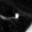
\includegraphics[width=\linewidth]{figures/heatmaps/ex1/sample_original.png}
        \caption*{Original 1}
    \end{subfigure}
    \begin{subfigure}[b]{0.18\textwidth}
        \centering
        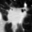
\includegraphics[width=\linewidth]{figures/heatmaps/ex2/sample_original.png}
        \caption*{Original 2}
    \end{subfigure}
    \begin{subfigure}[b]{0.18\textwidth}
        \centering
        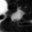
\includegraphics[width=\linewidth]{figures/heatmaps/ex3/sample_original.png}
        \caption*{Original 3}
    \end{subfigure}
    \begin{subfigure}[b]{0.18\textwidth}
        \centering
        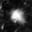
\includegraphics[width=\linewidth]{figures/heatmaps/ex4/sample_original.png}
        \caption*{Original 4}
    \end{subfigure}
    \begin{subfigure}[b]{0.18\textwidth}
        \centering
        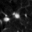
\includegraphics[width=\linewidth]{figures/heatmaps/ex5/sample_original.png}
        \caption*{Original 5}
    \end{subfigure}

    \vspace{2mm}

    % Second row: Fused model heatmaps
    \begin{subfigure}[b]{0.18\textwidth}
        \centering
        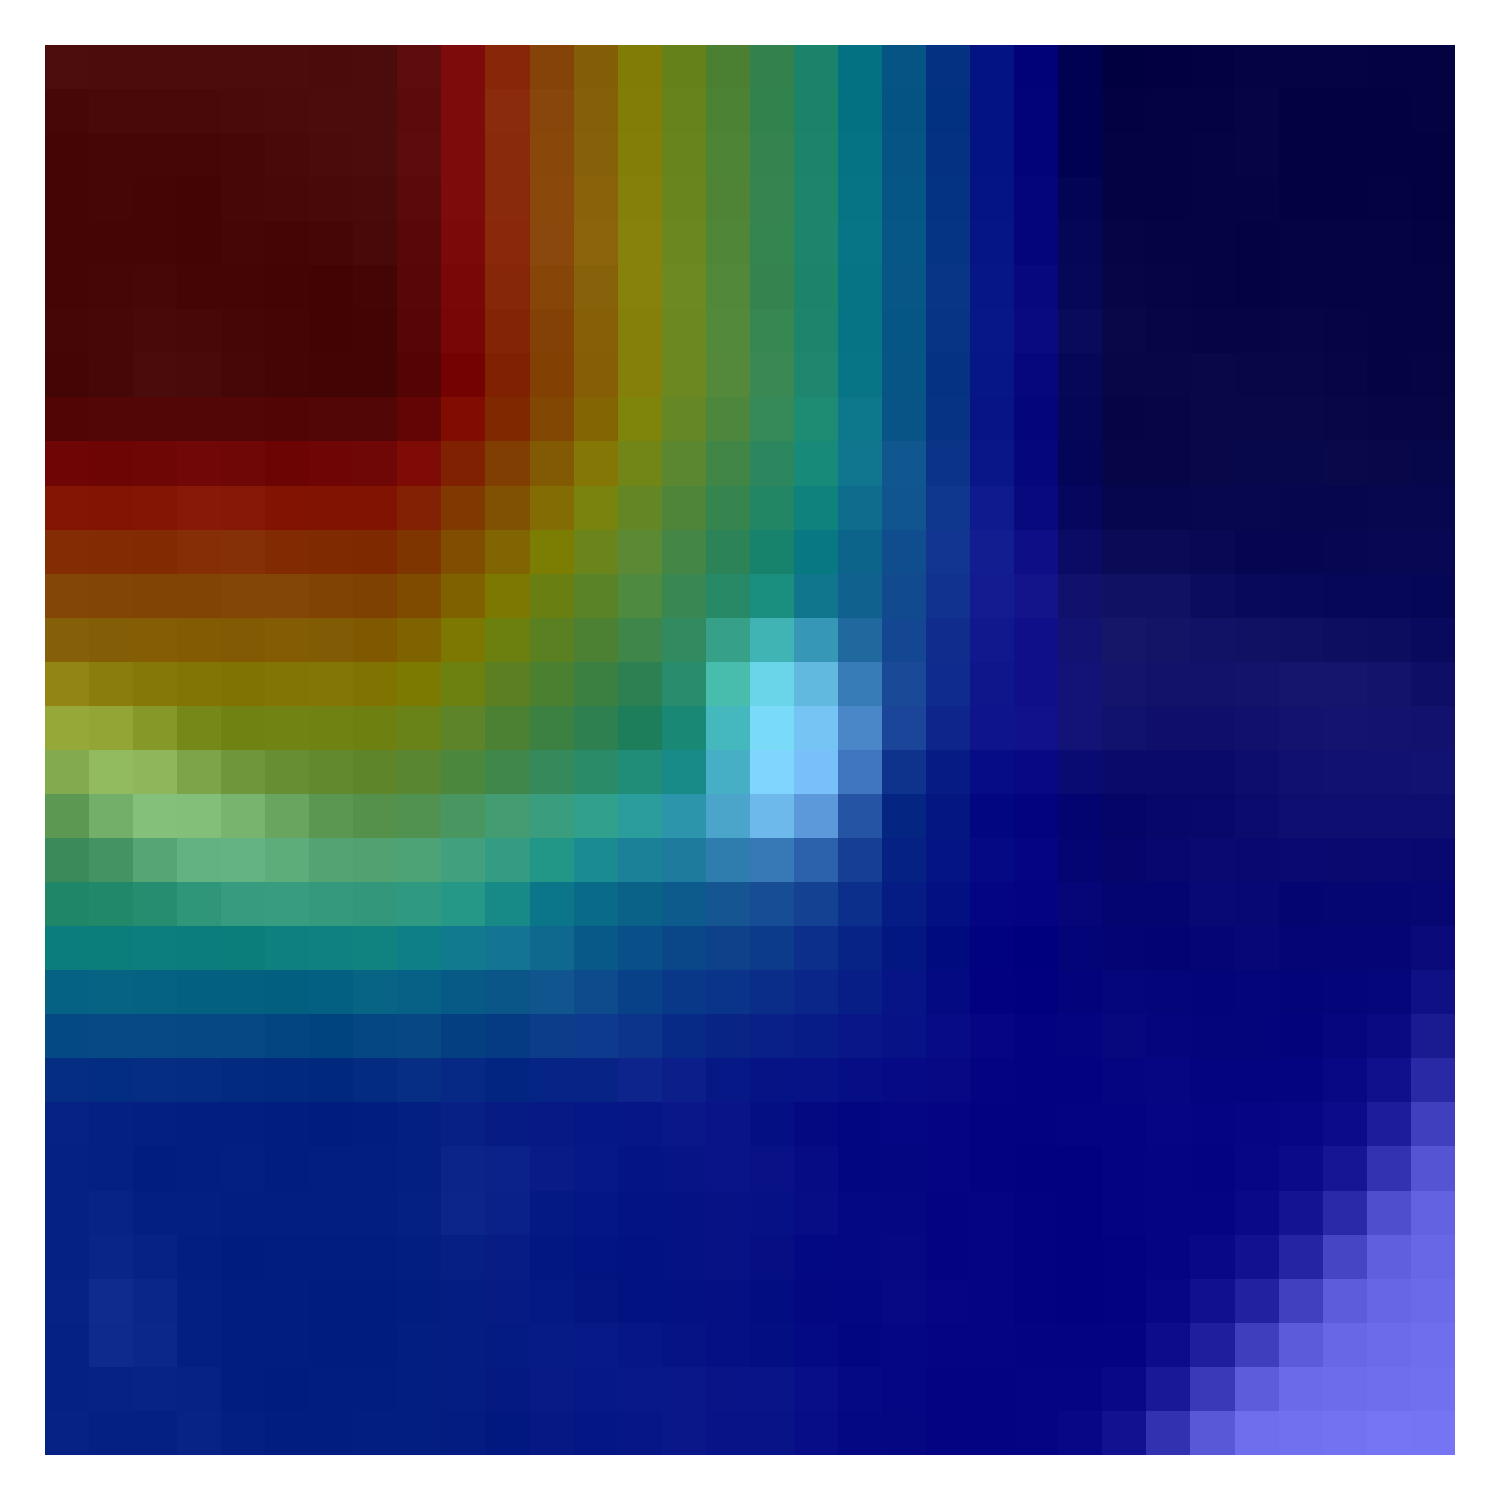
\includegraphics[width=\linewidth]{figures/heatmaps/ex1/sample_gradcam.png}
        \caption*{Fused 1}
    \end{subfigure}
    \begin{subfigure}[b]{0.18\textwidth}
        \centering
        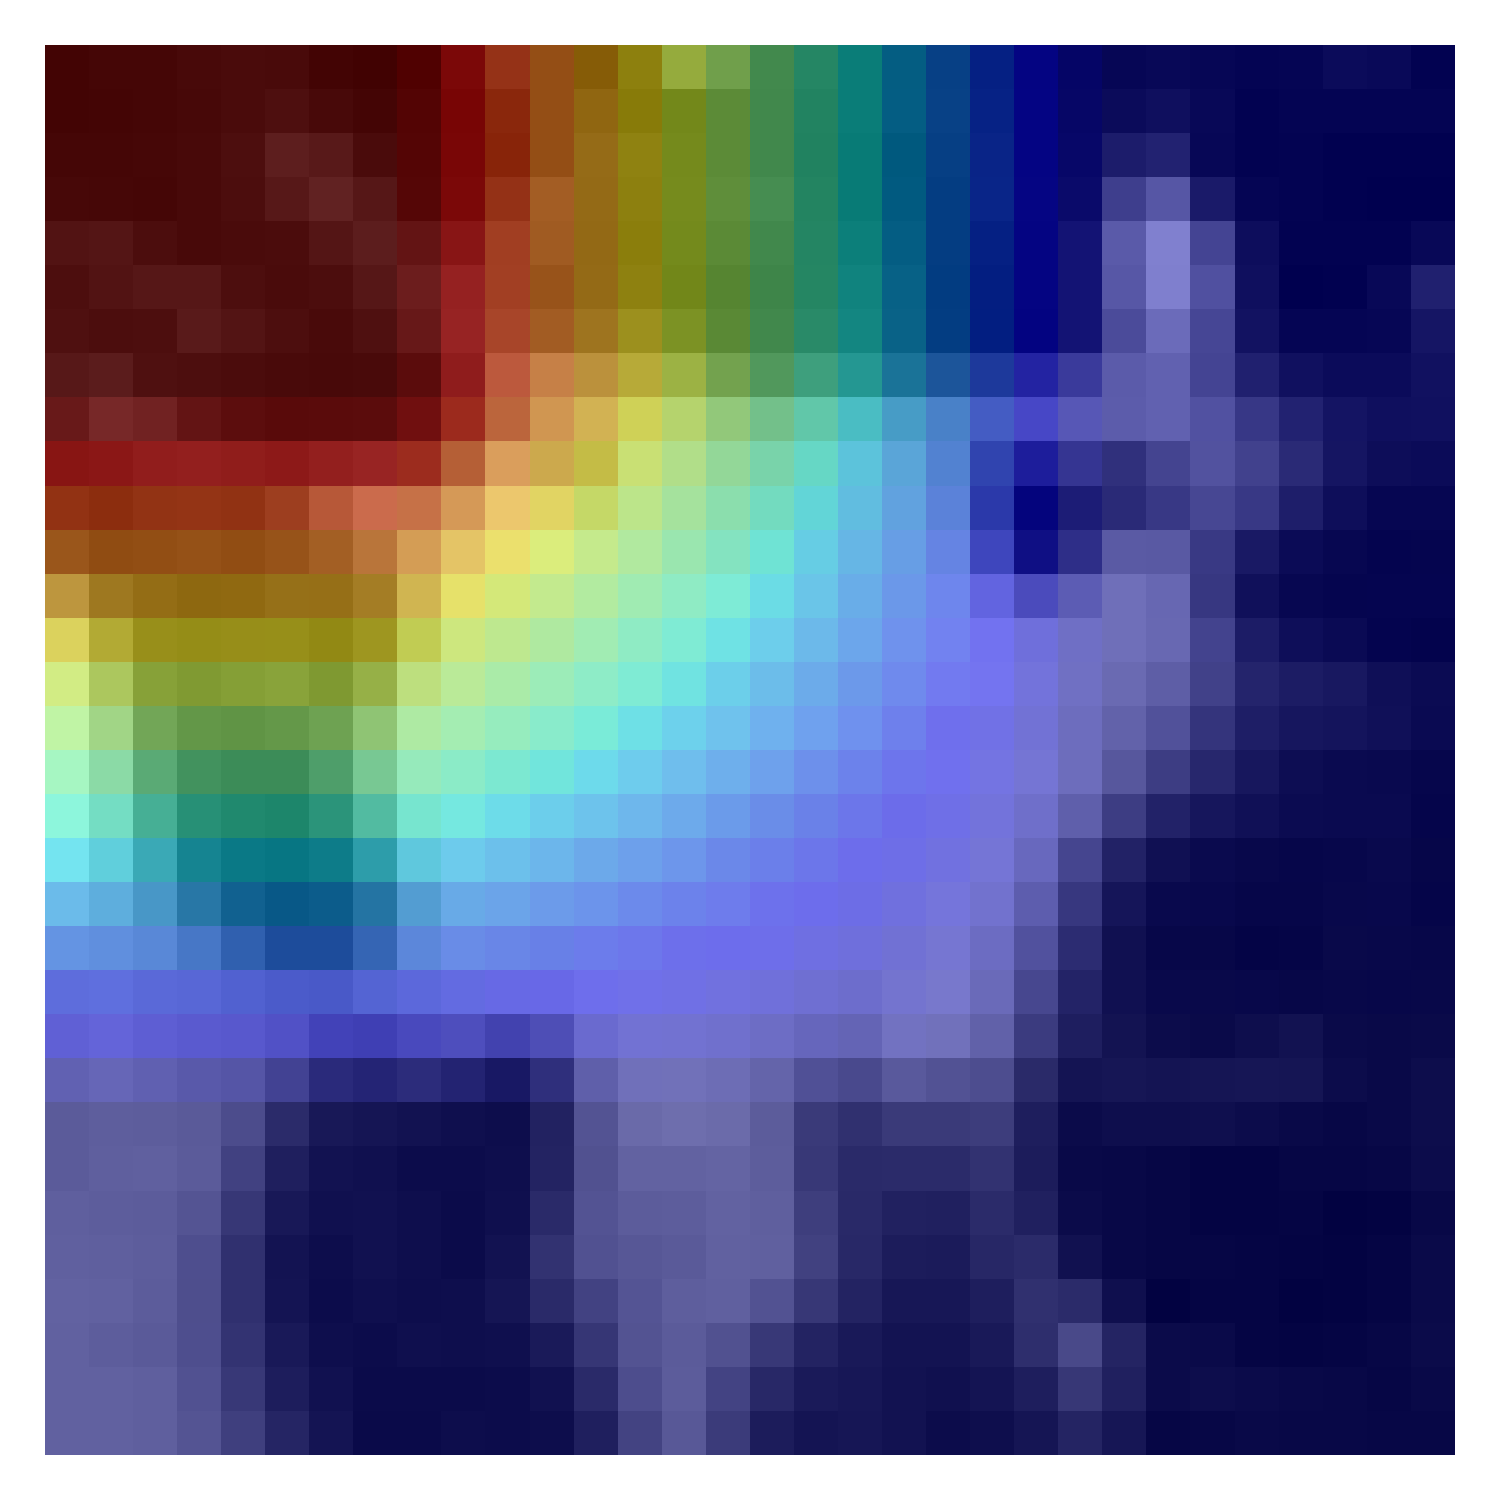
\includegraphics[width=\linewidth]{figures/heatmaps/ex2/sample_gradcam.png}
        \caption*{Fused 2}
    \end{subfigure}
    \begin{subfigure}[b]{0.18\textwidth}
        \centering
        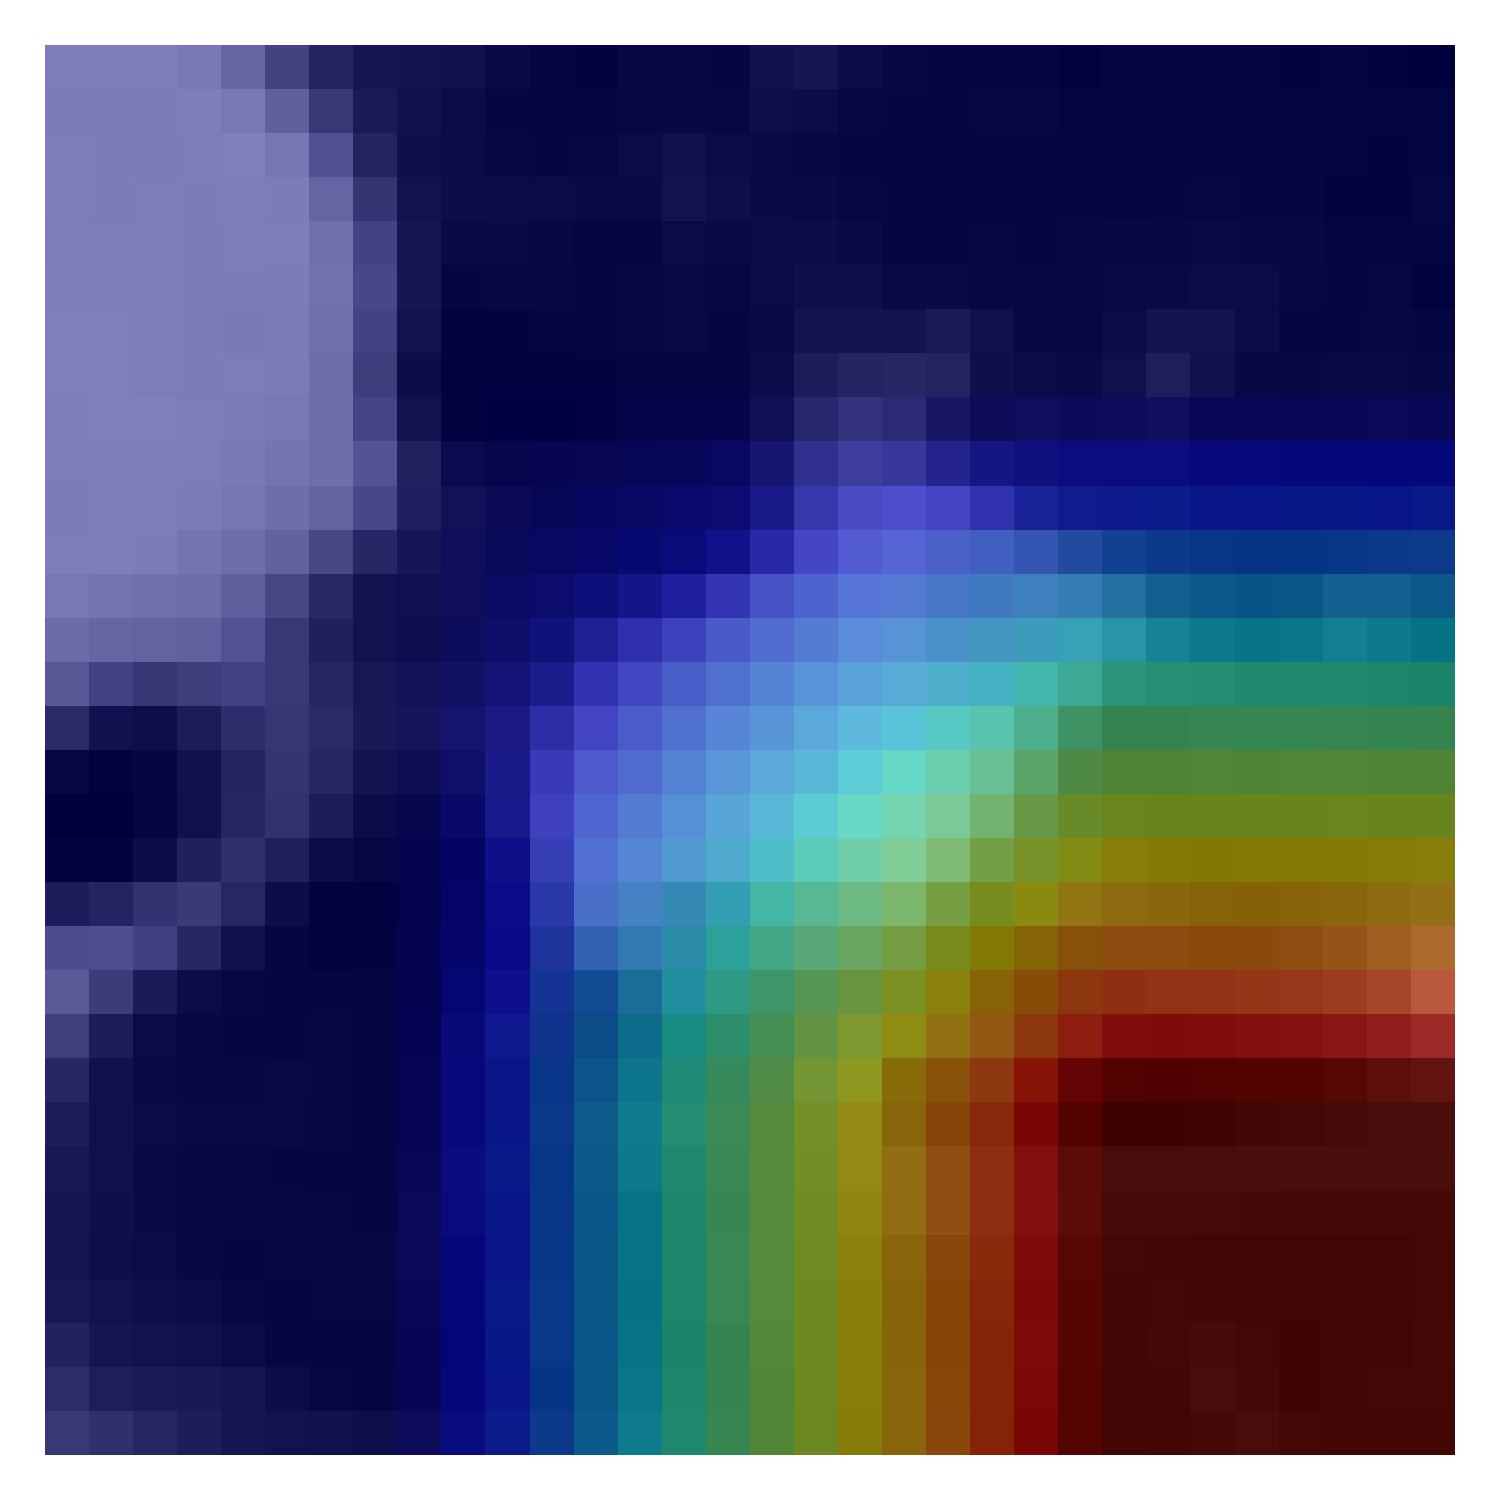
\includegraphics[width=\linewidth]{figures/heatmaps/ex3/sample_gradcam.png}
        \caption*{Fused 3}
    \end{subfigure}
    \begin{subfigure}[b]{0.18\textwidth}
        \centering
        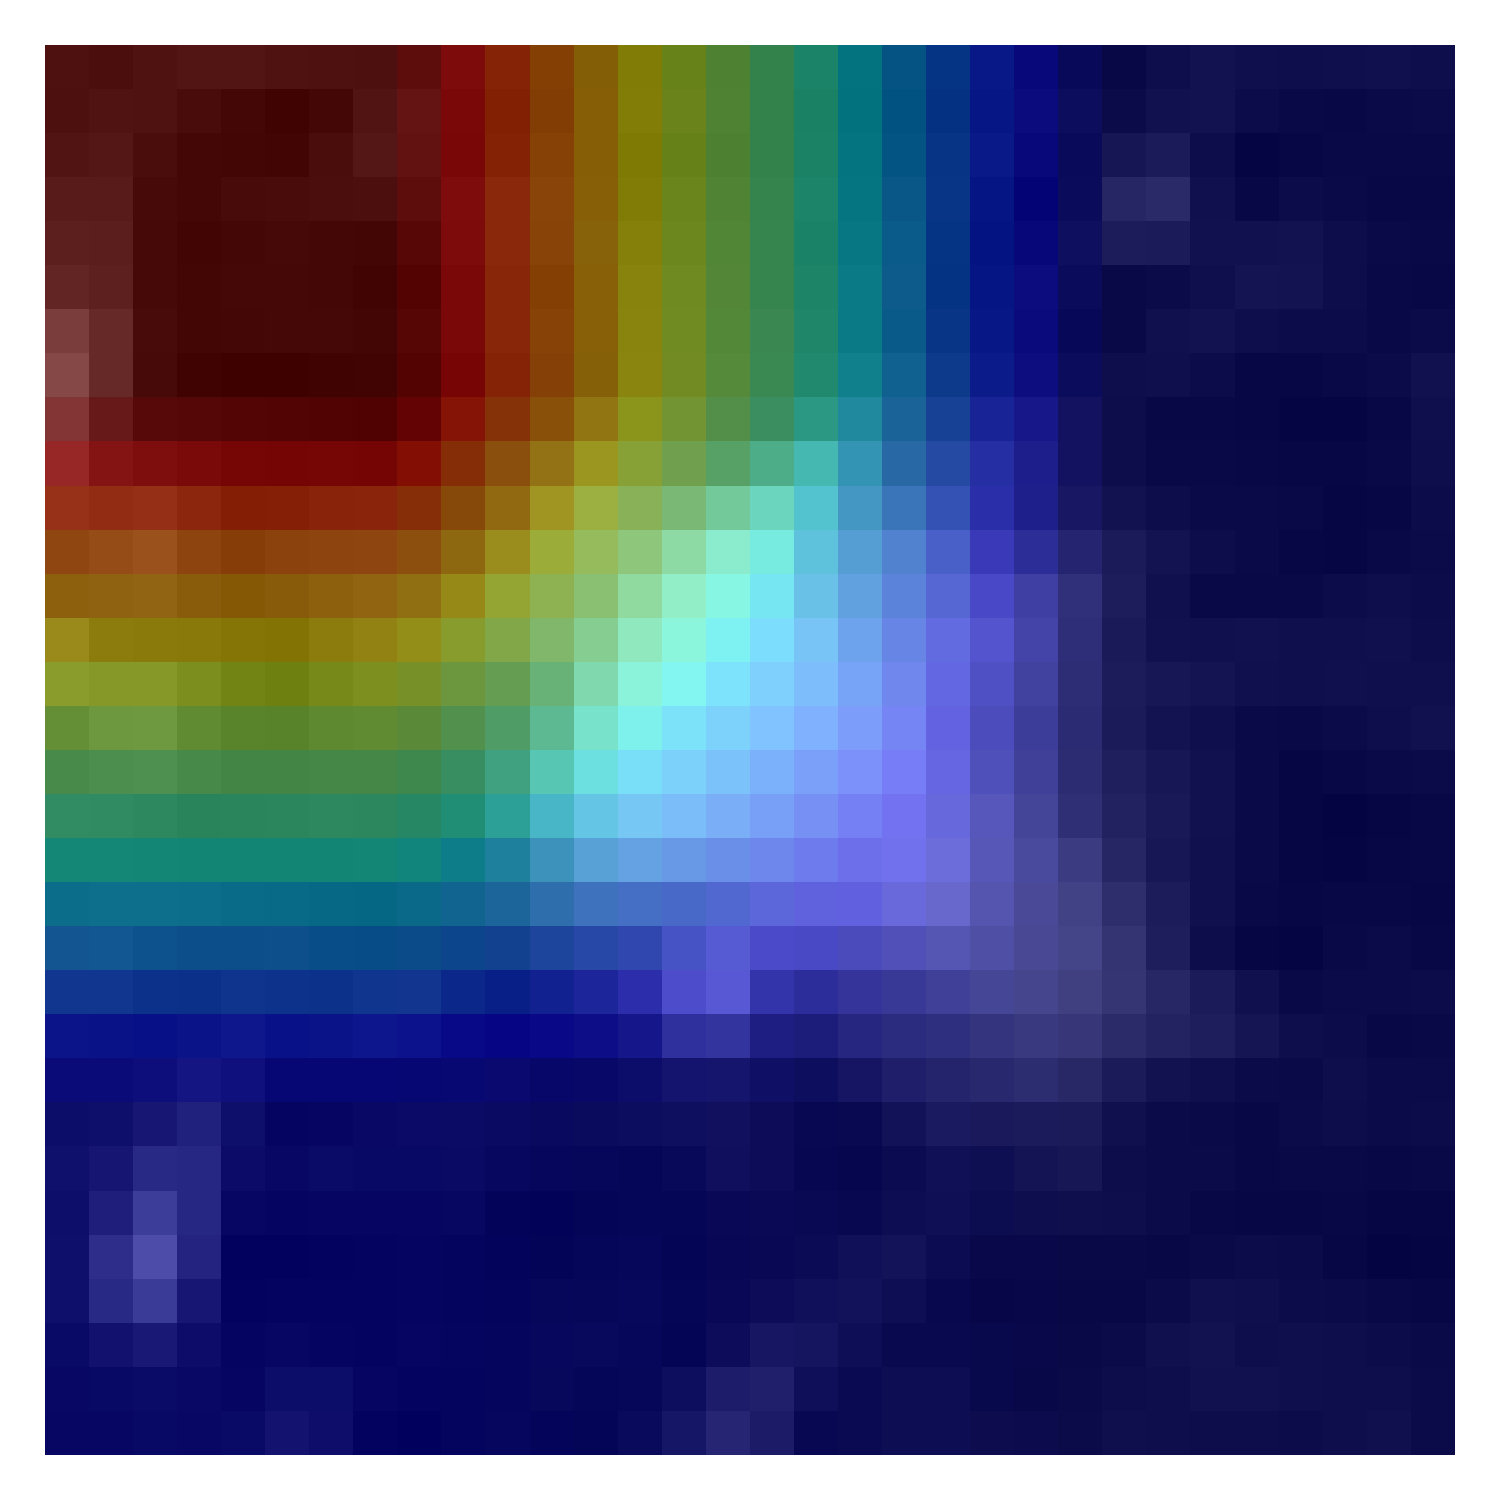
\includegraphics[width=\linewidth]{figures/heatmaps/ex4/sample_gradcam.png}
        \caption*{Fused 4}
    \end{subfigure}
    \begin{subfigure}[b]{0.18\textwidth}
        \centering
        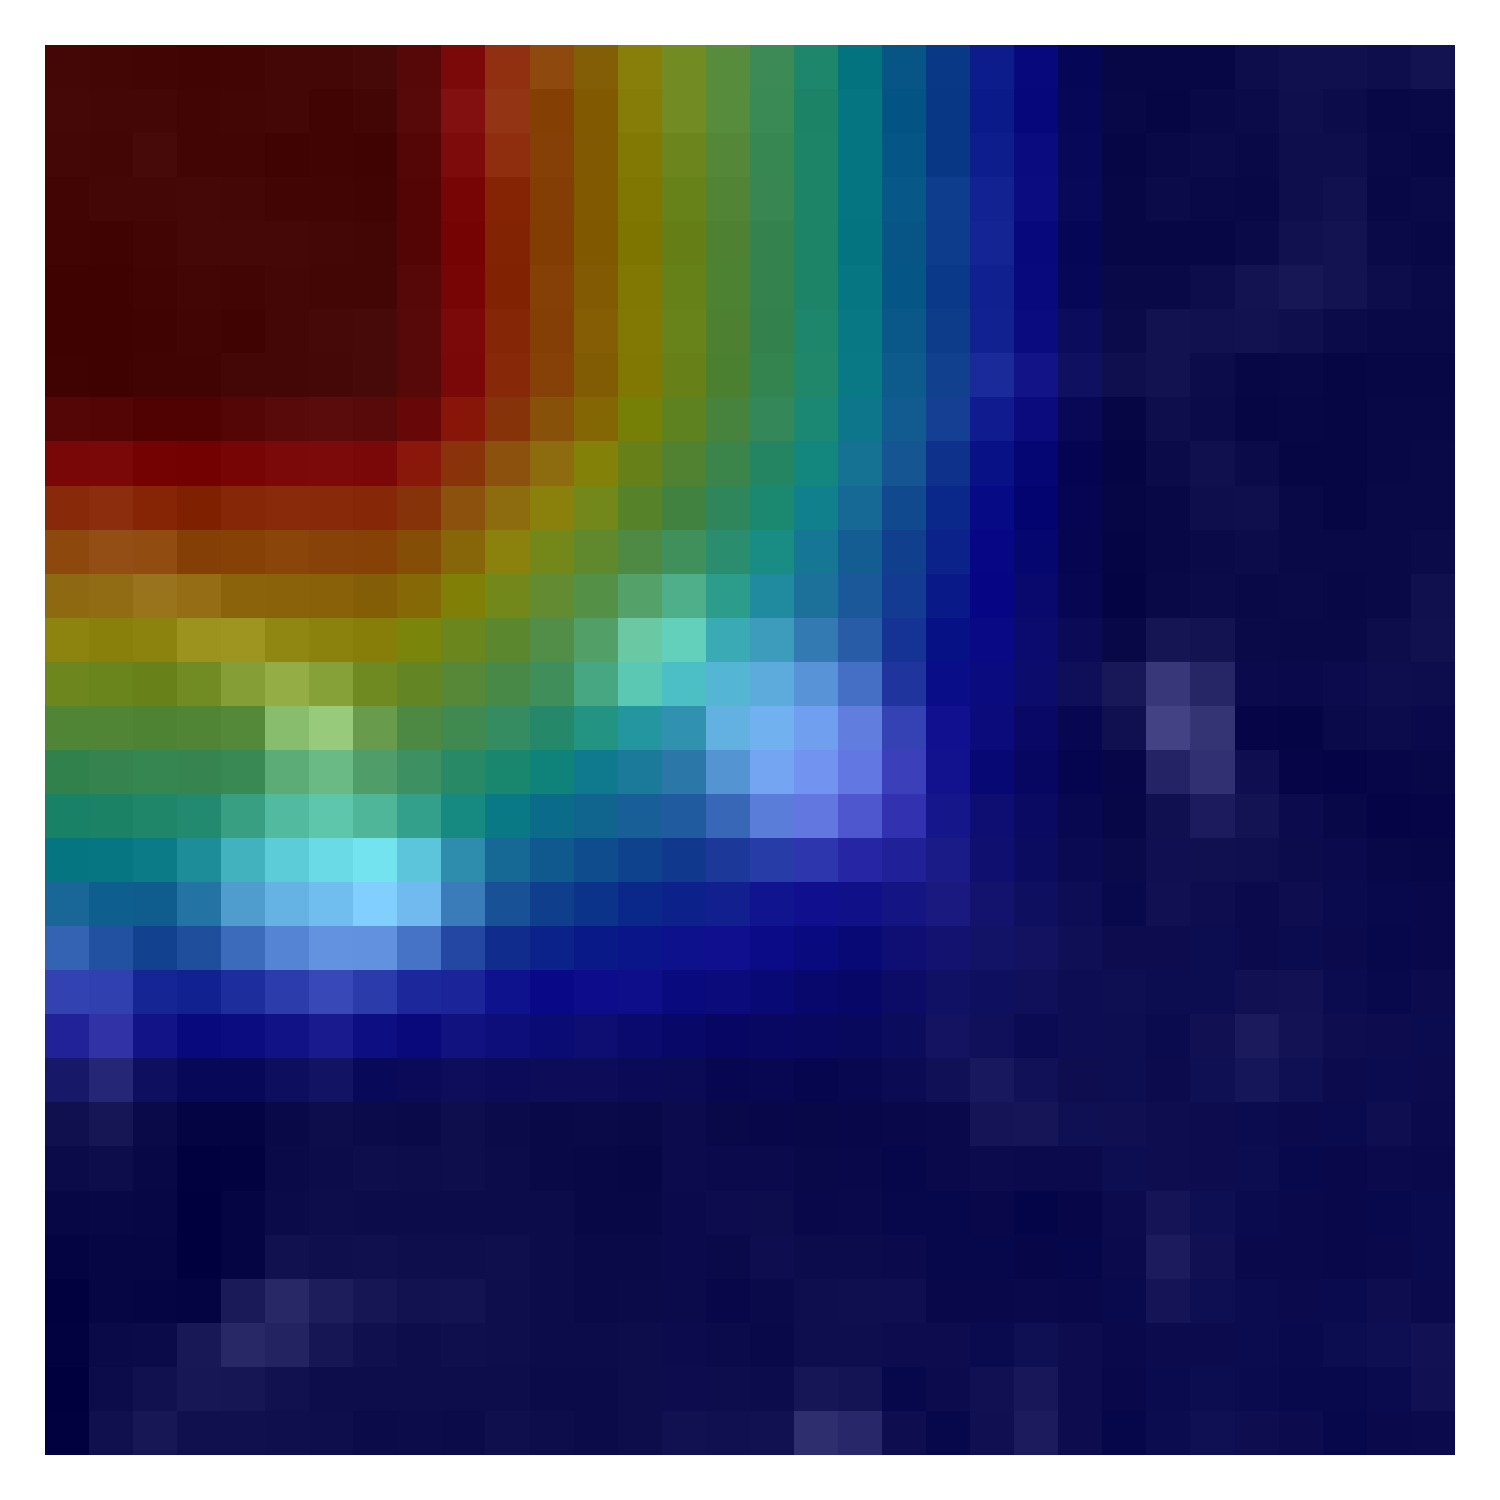
\includegraphics[width=\linewidth]{figures/heatmaps/ex5/sample_gradcam.png}
        \caption*{Fused 5}
    \end{subfigure}

    \vspace{2mm}

    % Third row: Non-Fused model heatmaps
    \begin{subfigure}[b]{0.18\textwidth}
        \centering
        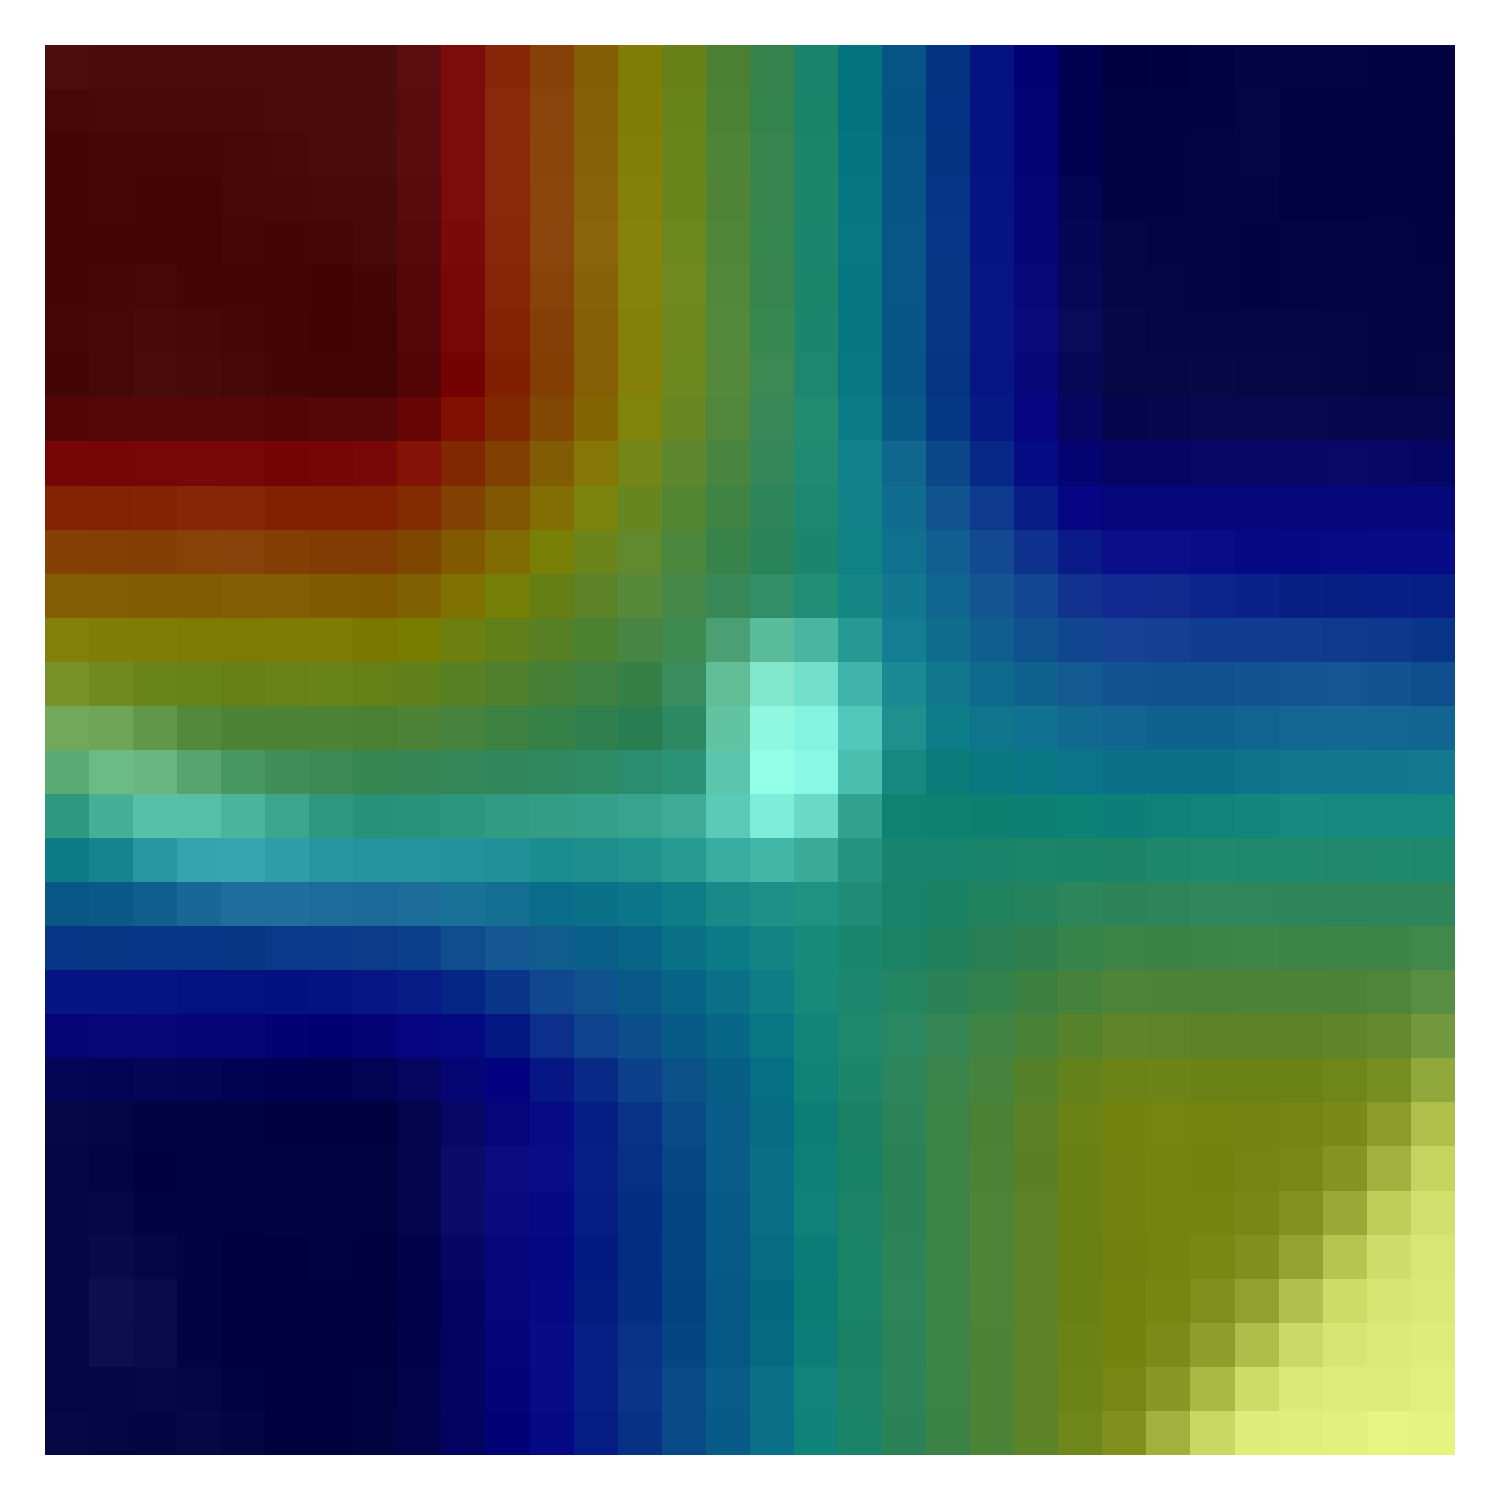
\includegraphics[width=\linewidth]{figures/heatmaps/ex1/sample_gradcam_non_fused.png}
        \caption*{Non-Fused 1}
    \end{subfigure}
    \begin{subfigure}[b]{0.18\textwidth}
        \centering
        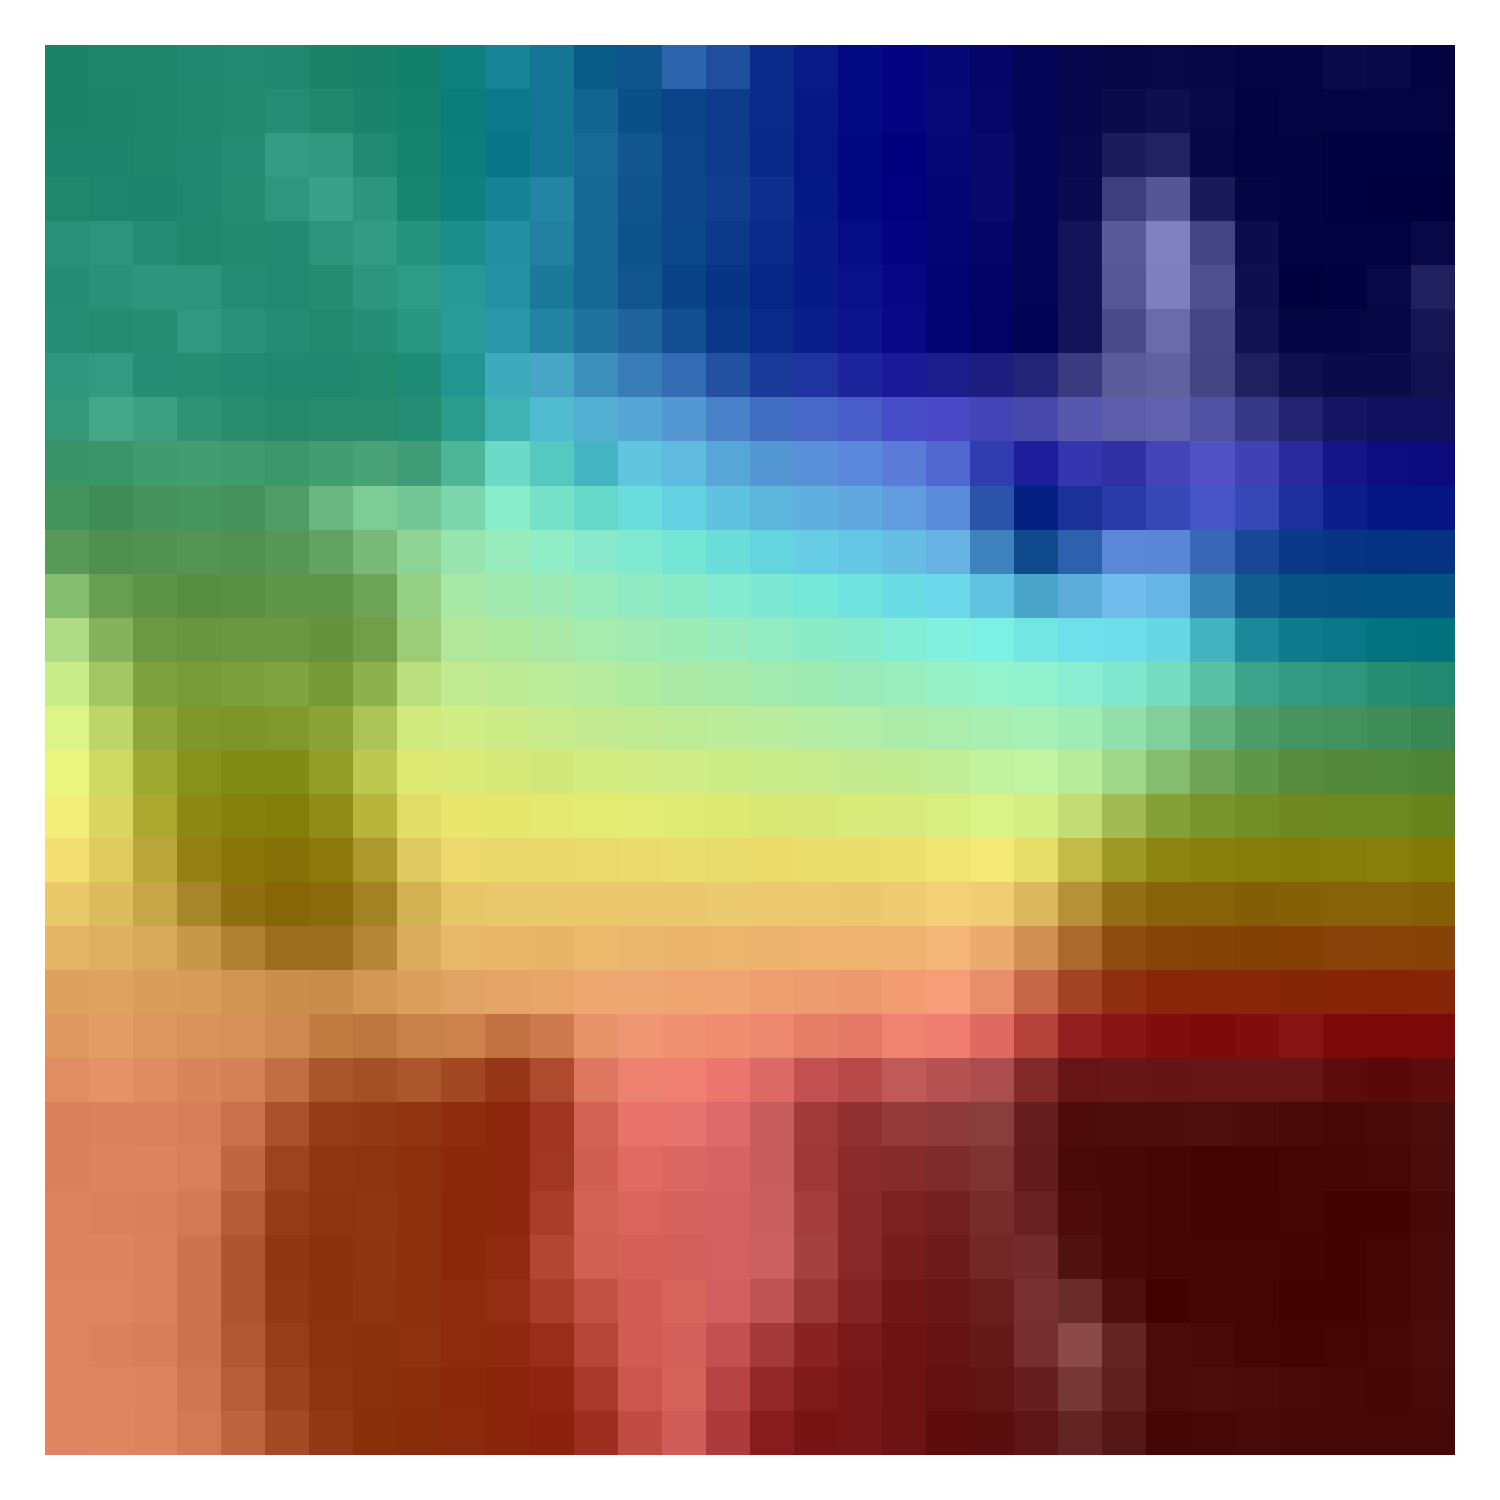
\includegraphics[width=\linewidth]{figures/heatmaps/ex2/sample_gradcam_non_fused.png}
        \caption*{Non-Fused 2}
    \end{subfigure}
    \begin{subfigure}[b]{0.18\textwidth}
        \centering
        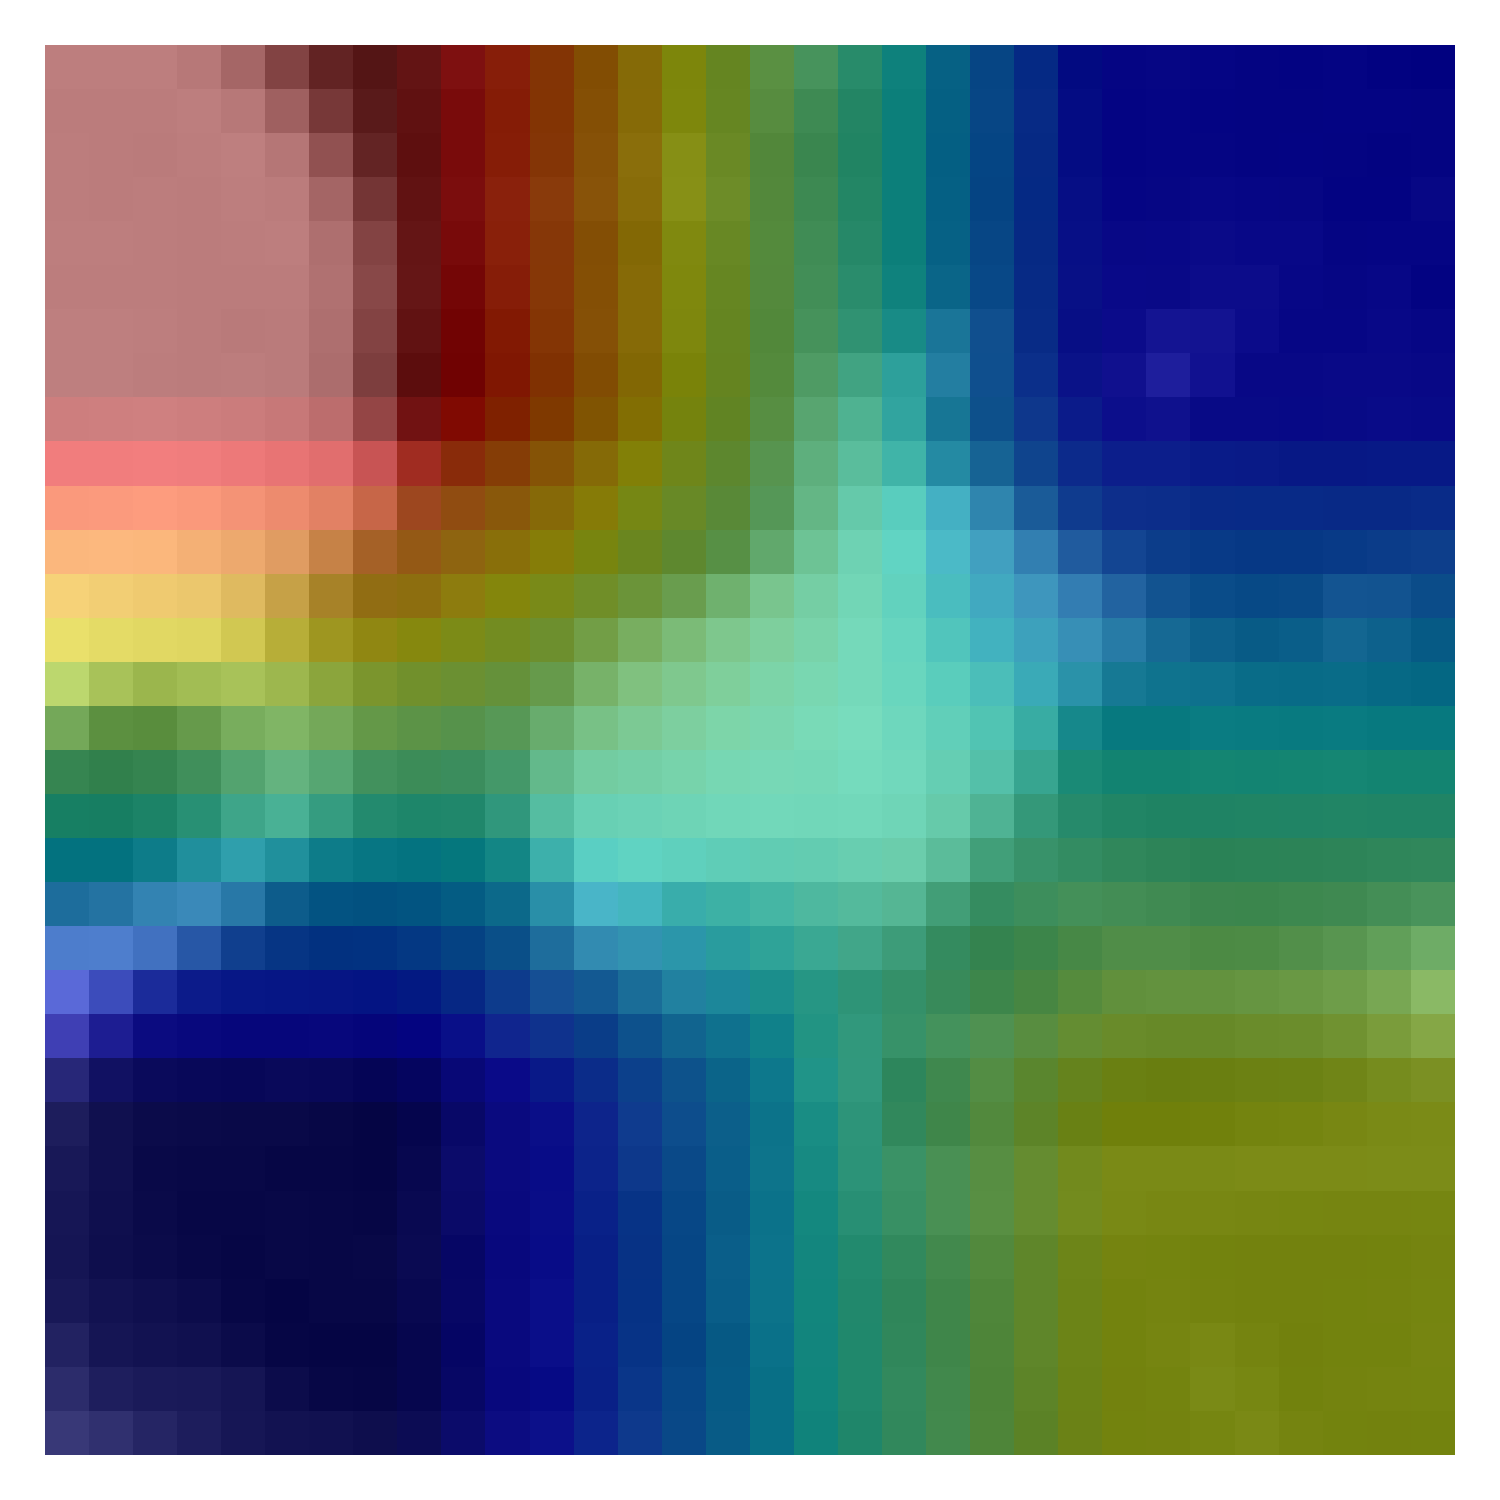
\includegraphics[width=\linewidth]{figures/heatmaps/ex3/sample_gradcam_non_fused.png}
        \caption*{Non-Fused 3}
    \end{subfigure}
    \begin{subfigure}[b]{0.18\textwidth}
        \centering
        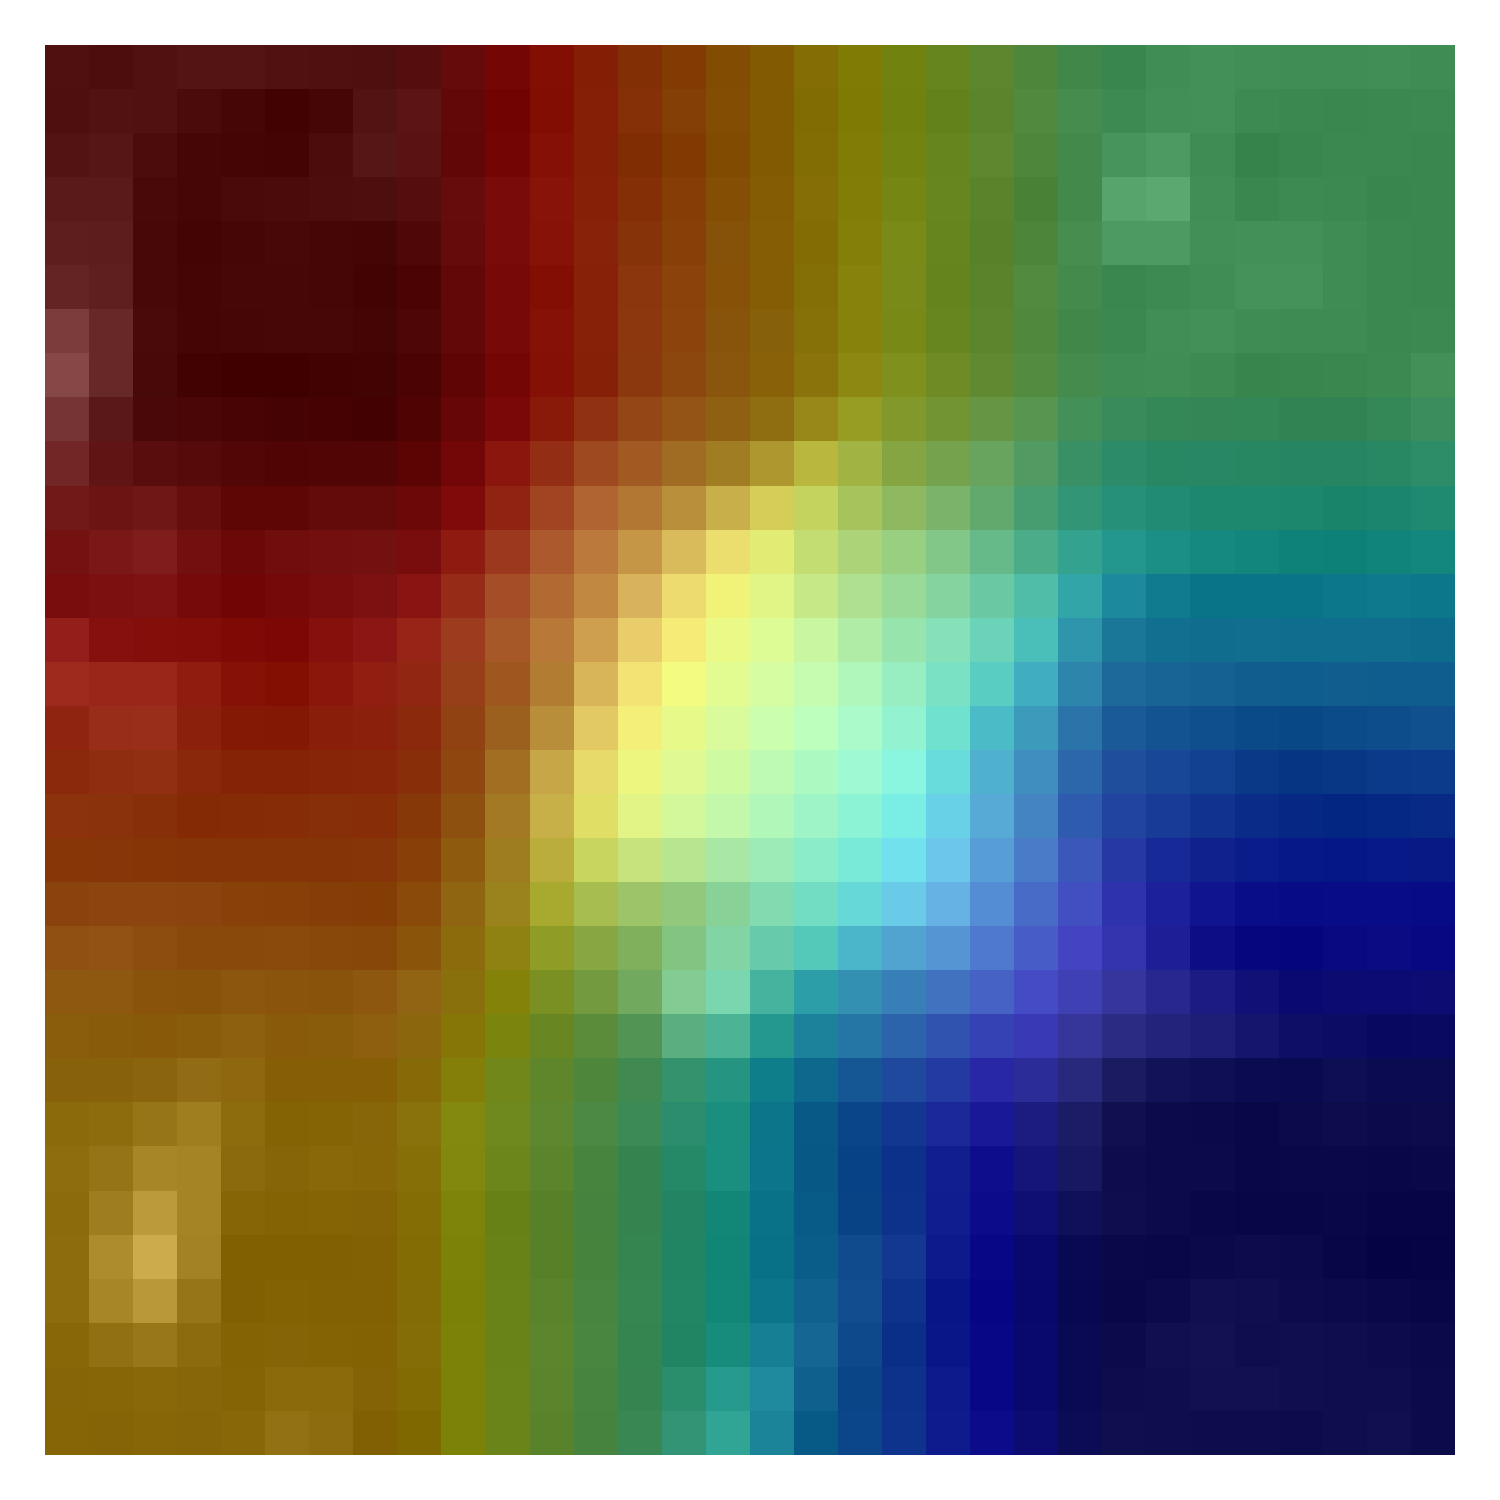
\includegraphics[width=\linewidth]{figures/heatmaps/ex4/sample_gradcam_non_fused.png}
        \caption*{Non-Fused 4}
    \end{subfigure}
    \begin{subfigure}[b]{0.18\textwidth}
        \centering
        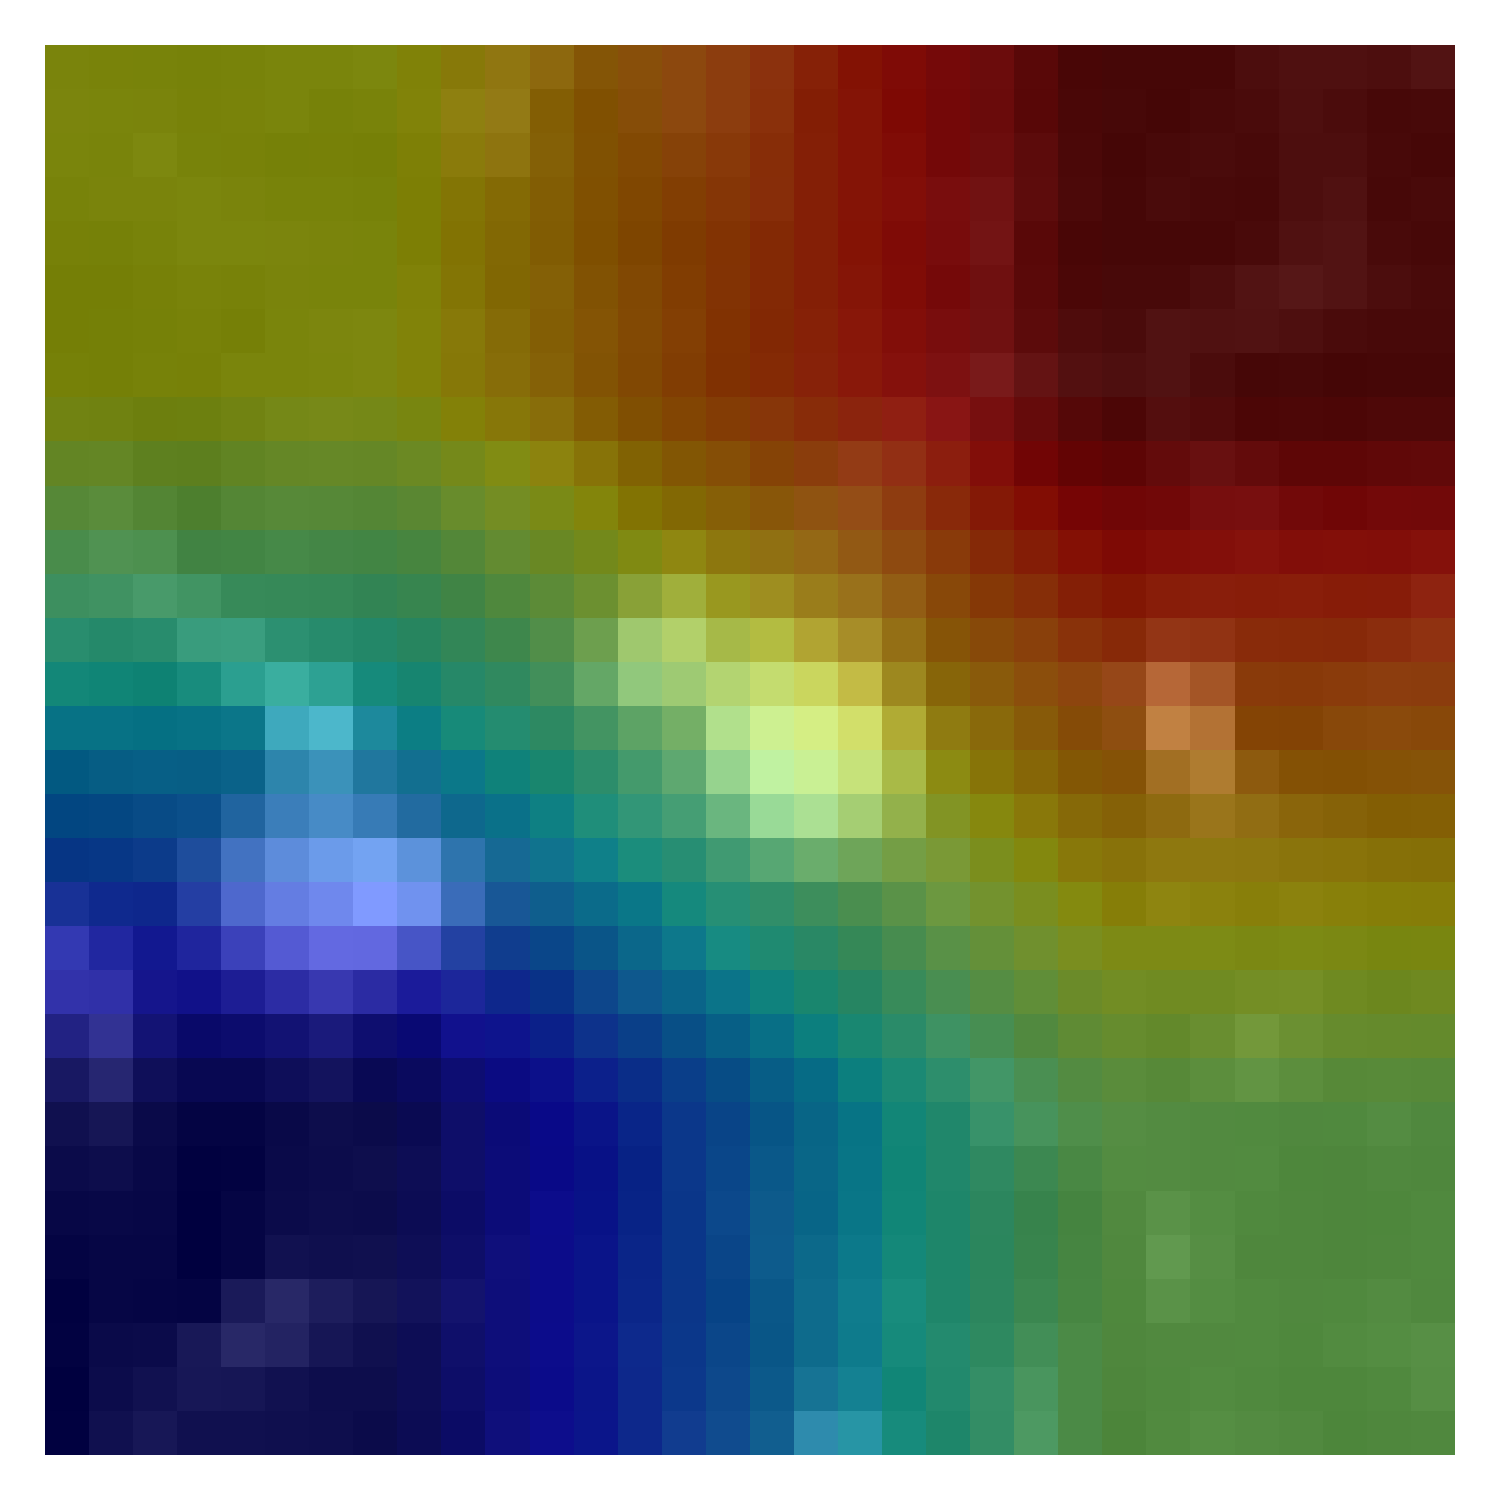
\includegraphics[width=\linewidth]{figures/heatmaps/ex5/sample_gradcam_non_fused.png}
        \caption*{Non-Fused 5}
    \end{subfigure}

    \caption[Grad-CAM Heatmap Comparison]{Comparison of Grad-CAM Heatmaps for five samples: Original images (top row), Fused model (middle row), and Non-Fused model (bottom row).}
    \label{fig:heatmap_grid}
\end{figure}


\subsection{SHAP}

\begin{figure}[htbp]
    \centering
    \begin{subfigure}[b]{0.45\textwidth}
        \centering
        \includegraphics[width=\linewidth]{figures/shap/true_positive/combined_shap_summary.png}
        \caption{True Positive}
    \end{subfigure}
    \begin{subfigure}[b]{0.45\textwidth}
        \centering
        \includegraphics[width=\linewidth]{figures/shap/false_positive/combined_shap_summary.png}
        \caption{False Positive}
    \end{subfigure}
    \vskip\baselineskip
    \begin{subfigure}[b]{0.45\textwidth}
        \centering
        \includegraphics[width=\linewidth]{figures/shap/false_negative/combined_shap_summary.png}
        \caption{False Negative}
    \end{subfigure}
    \begin{subfigure}[b]{0.45\textwidth}
        \centering
        \includegraphics[width=\linewidth]{figures/shap/true_negative/combined_shap_summary.png}
        \caption{True Negative}
    \end{subfigure}
    \caption[Local SHAP Analyses]{Local \ac{shap} Analyses for images representative of confusion matrix categories.}
    \label{fig:shap_analysis}
\end{figure}

Notably, \ac{shap} offers local, case-specific explanations, clarifying not only which features are significant on average but also how they specifically affect individual prediction outcomes within the confusion matrix.
The findings from the \ac{shap} analysis, illustrated in Figure~\ref{fig:shap_analysis}, offer valuable insights into the influence of specific radiomics features on the predictions made by the fused ResNet model across the four categories of the confusion matrix.

The results were derived by summing the \ac{shap} values for each feature. Higher positive \ac{shap} values indicate a greater influence on positive predictions, while negative values indicate influence on negative predictions.

Across all categories, the shape feature vector emerges as the primary contributor to the model's decisions. For both true positives and false negatives, the \ac{shap} values associated with Shape are significantly positive, suggesting that the presence of shape-related characteristics strongly reinforces the model's prediction of the positive class.

In the cases of false positives and true negatives, the \ac{shap} values for the Shape are strongly negative, indicating that when the shape feature influences the model towards the negative class, it does so with conviction. In contrast, the \ac{fof} and \ac{lbp} exhibit much smaller contributions across all categories: \ac{fof} has a minimal impact, whereas \ac{lbp} plays a slightly more significant role in negative-class predictions. 

This analysis confirms that integrating radiomics features with deep learning is most effective when shape features are included, as they significantly influence model predictions. The \ac{shap} analysis demonstrates that incorporating shape features enhances both interpretability and predictive power. In contrast, the contributions of \ac{fof} and \ac{lbp} are modest, suggesting that while multi-feature fusion offers complementary insights, the primary benefit comes from shape information. 